%!TEX root = ../msc_thesis.tex

\chapter{Artificial Neural Networks}
\label{ch:ann}

%%%%%%%%%%%%%%%%%%%%%%%%%%%%%%%%%%%%%%%%%%%%%%%%%%%%%%%%%%%%%%%%%%%%%%%%%%%%%%%%%%%%%%%%%%
%%%%%%%%%%%%%%%%%%%%%%%%%%%%%%%%%%%%%%%%%%%%%%%%%%%%%%%%%%%%%%%%%%%%%%%%%%%%%%%%%%%%%%%%%%
%%% ANNs
%%%%%%%%%%%%%%%%%%%%%%%%%%%%%%%%%%%%%%%%%%%%%%%%%%%%%%%%%%%%%%%%%%%%%%%%%%%%%%%%%%%%%%%%%%
%%%%%%%%%%%%%%%%%%%%%%%%%%%%%%%%%%%%%%%%%%%%%%%%%%%%%%%%%%%%%%%%%%%%%%%%%%%%%%%%%%%%%%%%%%

\section{Artificial Neural Networks}

The most basic, and perhaps the best known, type of Artificial Neural Network (ANN) is called a feed-forward neural network or multilayer perceptron (MLP). These models are basically a composition of non-linear functions of the data. We'll first introduce this concept in the ``classical'' way, as they were first introduced. Then we will skip to the Bayesian way.

Let's illustrate the multilayer perceptron with a simple example: consider that we want to model a continuous variable $y$ from a single feature $x$. A very simple model would be a linear regression, which models each observation $i$ as $y_i = \theta_0 + \theta_1 x_i$, and chooses the values of $\theta_0$ and $\theta_1$ that minimize some error function, most commonly the sum of the squared difference between the real values and the output of the model. ANNs go further and take non-linear transformations of this linear predictor with some function $\sigma(\cdot)$, such that $y_i = \theta_0^{[1]} +  \sum_{j = 1}^m \theta_j^{[1]} \sigma \left( \theta_0^{[0]} + \theta_j^{[0]} x_i \right)$, where $m$ is manually chosen beforehand. A common choice for $\sigma(\cdot)$, which is called the \textbf{activation function}, is the logistic function $\sigma(x) = (1 + e^{-x})^{-1}$
or the hyperbolic tangent $\tanh(\cdot)$. The values of parameters $\theta_k^{[0]}$ and $\theta_k^{[1]}$ for $k \in \left\{ 0, \ldots, m \right\}$ are also chosen to minimize certain error function. Figure \ref{fig:theory_ANN_diagram_01} shows these relationships in a graphic way for a model with $m = 3$ and where we define $a_{k, i} = \sigma \left( \theta_0^{[0]} + \theta_k^{[0]} x_i \right)$ for $k \in \left\{ 1, 2, 3 \right\}$.
This image doesn't explicitly show the parameters $\theta_0^{[0]}$ and $\theta_0^{[1]}$, which are usually called the \textbf{bias} parameters.

\begin{figure}[H]
    \centering
    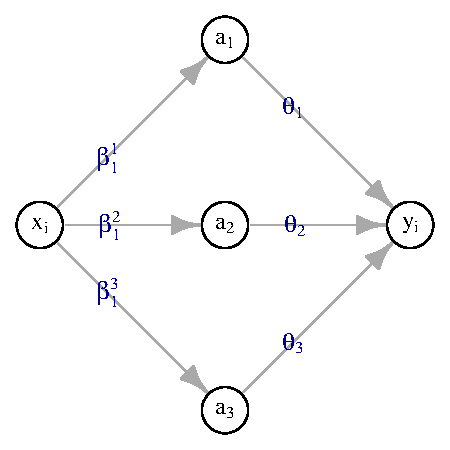
\includegraphics[width=0.5\textwidth]{plot_ANN_01.pdf}
    \caption{Diagram of a multilayer perceptron with $m = 3$.}
    \label{fig:theory_ANN_diagram_01}
\end{figure}

If the response variable $y$ happened to be a categorical variable, let's say binary, then one last transformation would have to be applied to map the model to the $\left[0, 1\right]$ interval and model $y$ as a probability. Then we would have

\begin{equation}
  y_i =
  \phi \left( \theta_0^{[1]} +  \sum_{j = 1}^m \theta_j^{[1]} \sigma \left( \theta_0^{[0]} + \theta_j^{[0]} x_i \right) \right) =
  \phi \left( \theta_0^{[1]} +  \sum_{j = 1}^m \theta_j^{[1]} a_{j,i} \right),
\end{equation}

with $\phi(\cdot)$ the logistic function to map from $\mathbb{R}$ to $\left[ 0, 1 \right]$. The choice of function $\phi(\cdot)$ depends on the nature of the response variable. As we saw previously, in the case of a continuous response variable, $\phi(\cdot)$ is the identity function.

We can establish a more complex model by taking linear combinations of non-linear functions of the previous result. Let's define
\begin{equation}
a_{k,i}^{[1]} = \sigma^{[1]} \left( \theta_{0}^{[1]} + \theta_k^{[0]} x_i \right)
\end{equation}

for $k \in \left\{ 1, \ldots, m \right\}$ and

\begin{equation}
  a_{k,i}^{[2]} = \sigma^{[2]} \left(  \theta_{0,k}^{[1]} + \sum_{j = 1}^m \theta_{j,k}^{[1]} a_{j,1}^{[0]}  \right)
\end{equation}

% \begin{equation}
% a_{k,i}^{[2]} = \theta_0^{j} +  \sum_{k = 1}^m \theta_k^{j} \sigma^{[2)} \left( \theta_0^{k} + \theta_1^{k} x_i \right) =
% \theta_0^{j} +  \sum_{k = 1}^m \theta_k^{j} a_{k,i}^{[1]}
% \end{equation}

for $k \in \left\{ 1, \ldots, r \right\}$, then

\begin{equation}
  y_i = \theta_0^{[2]} + \sum_{j = 1}^r \theta_j^{[2]} a_{j,i}^{[2]}
\end{equation}

where $r$, like $m$, is chosen beforehand. The values $m$ and $r$ are usually called the number of nodes or units of each layer. This is what is called a deeper model, because it has more layers. Notice that we have two different activation functions $\sigma^{[1]}(\cdot)$ and $\sigma^{[2]}(\cdot)$. Each layer can have a different function. The first one could be a sigmoid function and the second one a hyperbolic tangent, or vice versa, or they could both be the same function.

Figure \ref{fig:theory_ANN_diagram_02} shows this graphically with $m = 3$ and $r = 2$. Layers corresponding to $a_{k,i}^{[1]}$ for $k \in \left\{ 1, \ldots, m \right\}$ and $a_{k,i}^{[2]}$ for $k \in \left\{ 1, \ldots, r \right\}$ are called the \textbf{hidden layers}. So figure \ref{fig:theory_ANN_diagram_01} shows a multilayer perceptron with one hidden layer, and figure \ref{fig:theory_ANN_diagram_02} shows a multilayer perceptron with two hidden layers.


\begin{figure}[H]
    \centering
    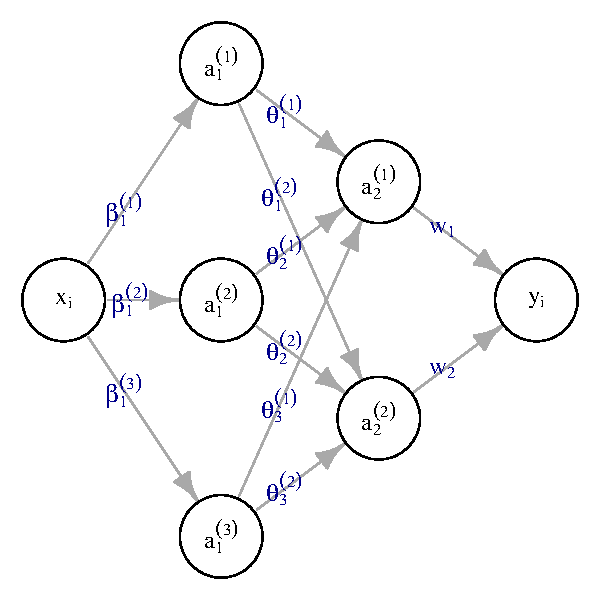
\includegraphics[width=0.6\textwidth]{plot_ANN_02.pdf}
    \caption{Diagram of a multilayer perceptron with two hidden layers, $m = 3$ and $r = 2$.}
    \label{fig:theory_ANN_diagram_02}
\end{figure}

Now that we have a grasp of how the MLP works, we can define it more generally. The notation used will be $y$ for the response variable $n$-dimensional vector, $y_i$ for the $i$-th element of $y$ and $X$ for the data matrix, such that $X \in \mathbb{R}^{n \times p}$, $x_i \in \mathbb{R}^p$ denotes the $i$-th row in $X$ and it represents the values of the features for the $i$-th element in the data and $x^{(k)} \in \mathbb{R}^n$ denotes the $k$-th column in $X$ and $x_i^{(k)}$ denotes the $k$-th column-wise element and the $i$-th row-wise element. Since a multilayer perceptron can have any integer number of hidden layers, we will denote the number of layers by $L$, the number of nodes of each layer $l$ by $n^{[l]}$ and the activation function for each layer $l$ by $\sigma^{[l]}(\cdot)$, for $l \in \left\{ 1, \ldots, L \right\}$. The activation function for the last layer will be denoted by $\phi(\cdot)$, as in the binary classification example. The parameter, or weight, that connects the $j$-th node from the $(l-1)$-th layer with the $k$-th node in the $l$-th layer is denoted by $\theta_{j,k}^{[l]}$ and, as before, $a_{k,i}^{[l]}$ denotes the result of the activation function corresponding to the $l$-th layer and the $i$-th observation, for $k \in \left\{ 1, \ldots, n^{[l]} \right\}$; where $\theta_{0,k}^{[l]}$ is the bias term of the $k$-th node in the $l$-th layer. That is,

\begin{equation}
  \label{eq:ann_act_funct_def}
  a_{k,i}^{[l]} = \sigma^{[l]} \left( \theta_{0,k}^{[l-1]} + \sum_{j = 1}^{n^{[l-1]}} \theta_{j,k}^{[l-1]} a_{j,i}^{[l-1]} \right)
\end{equation}

for $k \in \left\{ 1, \ldots, n^{[l]} \right\}$, $j \in \left\{ 1, \ldots, n^{[l-1]} \right\}$, $l \in \left\{ 1, \ldots, L \right\}$ and $i \in \left\{ 1, \ldots, n \right\}$.

To be consistent, $a_{k,i}^{[0]}$ is defined as $x_i^{[k]}$, and so, $a_{k}^{[0]} = x^{(k)} \in \mathbb{R}^n$; and $a_{0,i}^{[0]} = 1$ for all $i \in \left\{ 1, \ldots, n \right\}$, so $a_{0}^{[0]}$ is a vector of ones of dimension $n$ and $n^{[0]}$ is the number of features, i.e., $n^{[0]} = p$.

So, in general, a feed-forward neural network or multilayer perceptron with $L$ hidden layers is such that

\begin{equation}
  y_i = \phi \left( \theta_{0,1}^{[L]} +  \sum_{j = 1}^{n^{[L]}} \theta_{j,1}^{[L]} a_{k,i}^{[L]} \right),
\end{equation}

and where equation \eqref{eq:ann_act_funct_def} holds. As a way to summarize the whole notation, we will denote a multilayer perceptron with parameters $\Theta$ and data matrix $X$ as $\mathrm{MLP} \left(X, \Theta \right)$, where parameter $\Theta$ is a general way to refer to all parameters $\theta_{j,k}^{[l]}$ for $k \in \left\{ 1, \ldots, n^{[l]} \right\}$, $j \in \left\{ 1, \ldots, n^{[l-1]} \right\}$ and $l \in \left\{ 1, \ldots, L \right\}$.

Figure \ref{fig:theory_ANN_diagram_03} shows an example of an architecture with 2 hidden layers ($L = 2$), 4 features ($p = n^{[0]} = 4$), 3 nodes in the first hidden layer ($n^{[1]} = 3$) and 4 nodes in the second hidden layer ($n^{[2]} = 4$).

\begin{figure}[H]
    \centering
    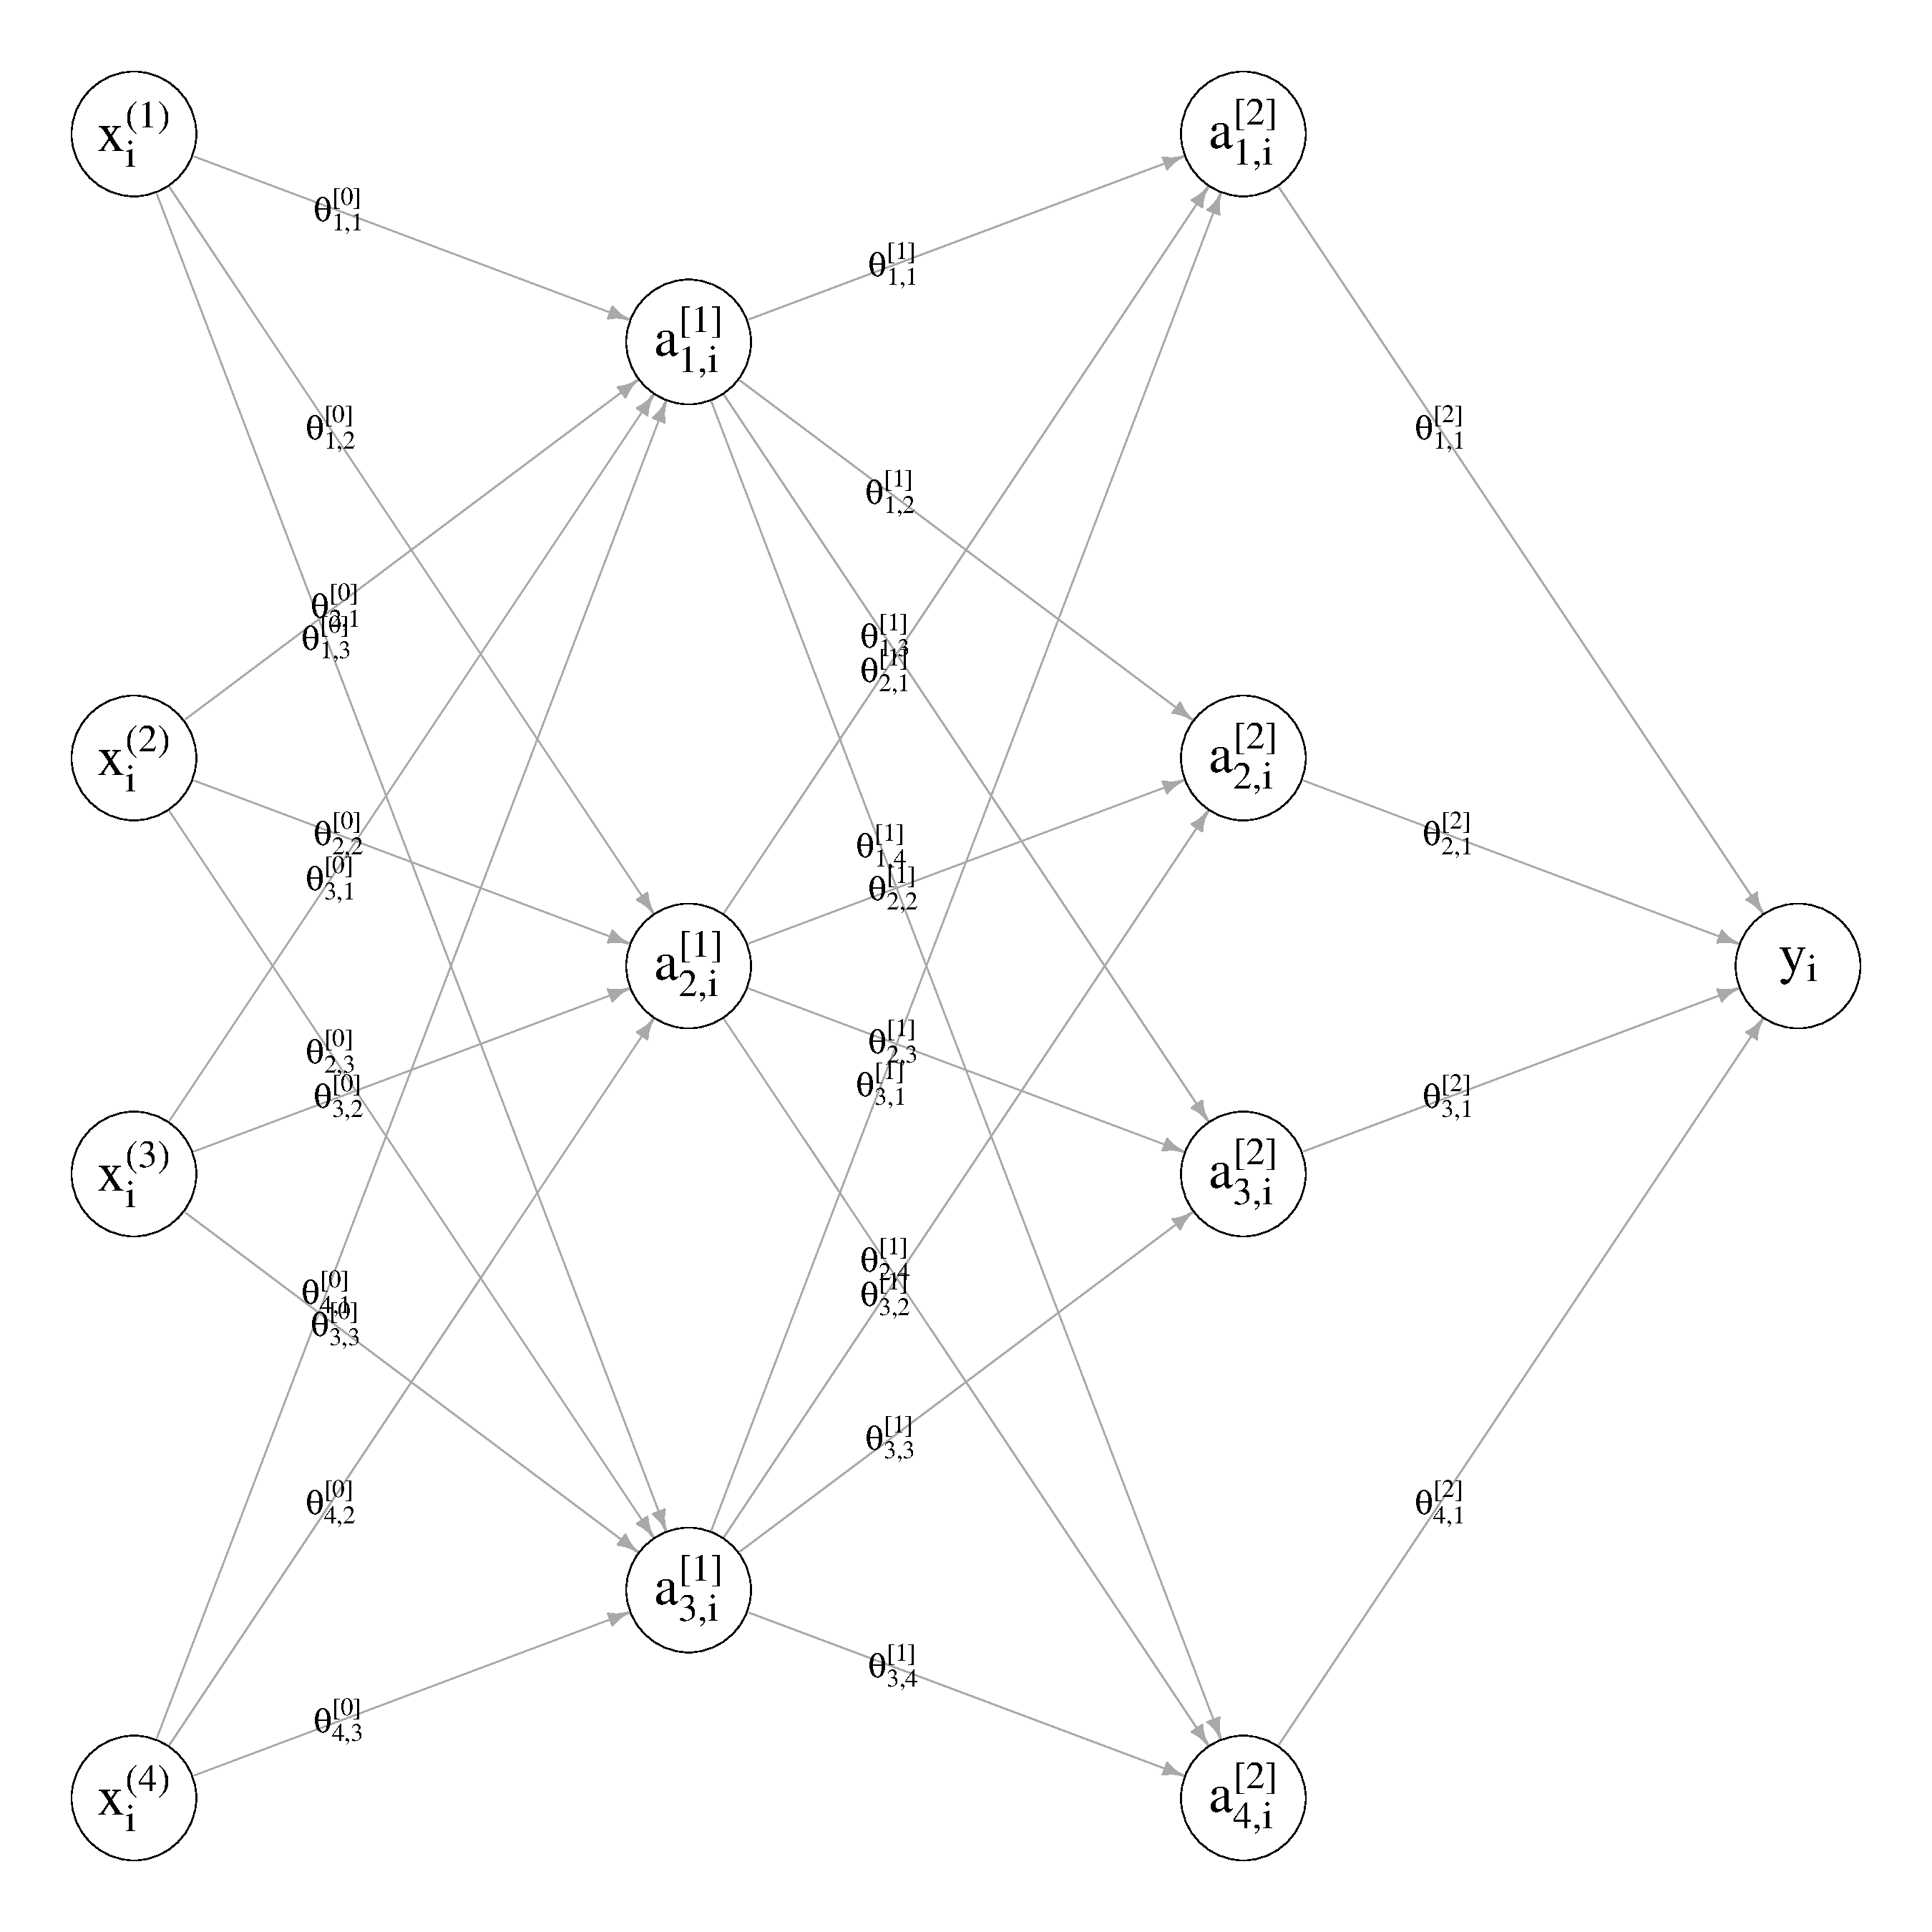
\includegraphics[width=0.95\textwidth]{plot_ANN_03.pdf}
    \caption{Diagram of a multilayer perceptron with two hidden layers using the general notation with $L = 2$, $p = n^{[0]} = 4$, $n^{[1]} = 3$ and $n^{[2]} = 4$.}
    \label{fig:theory_ANN_diagram_03}
\end{figure}

As mentioned before, the values of the parameters in the network are chosen so that they minimize a certain error function. In the continuous case, the commonly called \textbf{squared loss} is often used, defined as the sum of the squared difference between the real values and the output of the model, which is also equivalent to the maximization of a Gaussian likelihood function. This loss function is mathematically defined as

\begin{equation}
  L(\Theta) = \sum_{i = 1}^n \left[ y_i - \hat{y}_i \right]^2
\end{equation}

where $\hat{y_i}$ is the output of the model for the $i$-th observation of the data and the feature vector $x_i$ and $\Theta$ is the vector of all parameters in the model.

In the case of a binary classification problem, a very commonly used loss is the so-called \textbf{cross-entropy} loss, which is the result of maximizing the log-likelihood of independent Bernoulli response variables. In the context of loss function, it is defined as

\begin{equation}
  \label{eq:binary_cross_entropy_loss}
  L(\Theta) = - \sum_{i = 1}^n \left[ y_i \log{\left( \hat{y}_i \right)} + (1 - y_i) \log{\left( 1 - \hat{y}_i \right)} \right].
\end{equation}

In the case of a multiple classification problem, equation \eqref{eq:binary_cross_entropy_loss} is extended for more classes using the same maximum likelihood idea. In a $k$ class classification problem, the loss is defined as

\begin{equation}
  L(\Theta) = - \sum_{i = 1}^n \left[ \sum_{j = 1}^k y_{i,j} \log{\left( \hat{y}_{i,j} \right)}  \right]
\end{equation}

where $y_{i,j} = 1$ if the $i$-th training point belongs to the $j$-th class and $\hat{y}_{i,j}$ is the model's predicted probability of the $i$-th training point belonging to the $j$-th class.

In the Bayesian approach, we first assign prior distributions to each of the parameters and specify a conditional distribution to the response variable $y$. For example, in the continuous case, it is common to assign a Gaussian conditional distribution to $y$, such that

\begin{equation}
  y | \Theta, X \sim \normaldist{\mathrm{MLP}(X, \Theta)}{\sigma^2}
\end{equation}

where $\mathrm{MLP}(X, \Theta)$ denotes the architecture of a multilayer perceptron with parameters $\Theta$ and data matrix $X$. Since the $\Theta$ parameters can be any real value, it is also common to assign a Gaussian distribution to them, so that the prior distribution is such that

\begin{equation}
  \theta_{i,k}^{[l]} \sim \normaldist{\mu_{i,k}^{[l]}}{\sigma_{i,k}^{[l]}}.
\end{equation}

Parameters $\mu_{i,k}^{[l]}$ and $\sigma_{i,k}^{[l]}$ are chosen to reflect the prior knowledge that we may have about the values of the parameters $\theta_{i,k}^{[l]}$. If we have no prior knowledge, then a vague prior can be used.

In contrast to classical neural networks where parameters $\Theta$ are chosen so that they minimize an error function, in Bayesian neural networks we wish to update our knowledge on the parameters $\Theta$ given the data $X$ and $y$. This is achieved with Bayes' theorem in the following way

\begin{equation}
  \prob{\Theta | X, y} = \frac{\prob{y | \Theta, X} \prob{\Theta | X}}{\prob{y | X}}.
\end{equation}

%In our example, $\prob{X | \Theta} = \normalfunc{X}{\mathrm{MLP}(X, \Theta)}{\sigma^2}$ and $\prob{\Theta} = \normalfunc{\Theta}{[]}$
In our example, $\prob{y | \Theta, X}$ and $\prob{\Theta | X}$ are the joint density functions of Gaussian random variables with their corresponding parameter values.

To make predictions in the Bayesian case, we use the posterior predictive distribution defined in equation \eqref{eq:post_pred_dist}.


%%%%%%%%%%%%%%%%%%%%%%%%%%%%%%%%%%%%%%%%%%%%%%%%%%%%%%%%%%%%%%%%%%%%%%%%%%%%%%%%%%%%%%%%%%
%%%%%%%%%%%%%%%%%%%%%%%%%%%%%%%%%%%%%%%%%%%%%%%%%%%%%%%%%%%%%%%%%%%%%%%%%%%%%%%%%%%%%%%%%%
%%% CNNs
%%%%%%%%%%%%%%%%%%%%%%%%%%%%%%%%%%%%%%%%%%%%%%%%%%%%%%%%%%%%%%%%%%%%%%%%%%%%%%%%%%%%%%%%%%
%%%%%%%%%%%%%%%%%%%%%%%%%%%%%%%%%%%%%%%%%%%%%%%%%%%%%%%%%%%%%%%%%%%%%%%%%%%%%%%%%%%%%%%%%%

\section{Convolutional Neural Networks}

Convolutional Neural Networks (CNNs) are neural networks with a quite particular architecture and are widely used in computer vision problems, such as image classification or object detection in a video. They were introduced by \citeauthor{lecun1989generalization} in \citeyear{lecun1989generalization} as a way to constrain the number of parameters needed to perform automatic image classification \cite{lecun1989generalization}. The main idea is that in images, pixels close to each other tend to be similar, whereas pixels far away from each other tend to be different. This notion of proximity is used by CNN's architecture, and leverages three concepts: sparse interactions, parameter sharing and equivariant representations \cite[p.~335]{bengio2015deep}.

\begin{itemize}
  \item Sparse interactions: In MLPs, every unit is connected to all other units in the next layer, but in CNNs, only a small number of units is connected to another small number of units. This means fewer parameters and, hence, less memory usage and faster computation.
  \item Parameter sharing: Different units share the same set of parameters. The same convolution is used many times in the image and, thus, the number of parameters is further reduced.
  \item Equivariant representations: The architecture of CNNs provides equivariance in translations, meaning that if the input is changed, the output is changed in the same fashion. For example: in an image, if an object is moved in the input, its representation will be moved in the same way in the output.
\end{itemize}

\subsection{Convolution operation}

The base of CNNs is the convolution operation, which will be described assuming an image. Let's assume that we have an image represented as a $m \times n$ matrix $I$, with $I_{i,j}$ represents the pixel in the $i$-th row and $j$-th column as such

\begin{equation}
  I =
    \begin{bmatrix}
      I_{1,1} & I_{1,2} & I_{1,3} & \dots  & I_{1,n} \\
      I_{2,1} & I_{2,2} & I_{2,3} & \dots  & I_{2,n} \\
      \vdots & \vdots & \vdots & \ddots & \vdots \\
      I_{m,1} & I_{m,2} & I_{m,3} & \dots  & I_{m,n}
    \end{bmatrix}.
\end{equation}

The convolution operation uses another matrix called a \textbf{filter} or a \textbf{kernel}, with dimensions $p \times r$. This matrix must be of a lower dimension than the image, that is, $p < m$ and $r < n$. Let's denote the filter as matrix $K$ as such

\begin{equation}
  K =
    \begin{bmatrix}
      \theta_{1,1} & \theta_{1,2} & \theta_{1,3} & \dots  & \theta_{1,q} \\
      \theta_{2,1} & \theta_{2,2} & \theta_{2,3} & \dots  & \theta_{2,q} \\
      \vdots & \vdots & \vdots & \ddots & \vdots \\
      \theta_{p,1} & \theta_{p,2} & \theta_{p,3} & \dots  & \theta_{p,q}
    \end{bmatrix}.
\end{equation}

The convolution operation between $I$ and $K$ is denoted as $I * K$, and its result is another matrix $S$, for which each element is defined as

\begin{equation}
  \label{eq:2d_conv_def}
  S_{i,j} = (I * K)_{i,j} = \sum_{k} \sum_{l} I_{i+k-1,j+l-1} K_{k, l}.
\end{equation}

An example of this is shown in figure \ref{fig:conv_example}, in which $I$ is a $7 \times 7$ image matrix and the kernel is a $3 \times 3$ matrix. The result is a $5 \times 5$ matrix in which element is computed using equation \eqref{eq:2d_conv_def}. For instance, the element on the first row and fourth column of the result matrix, that is, $S_{1,4}$ is computed as

\begin{equation}
  \begin{split}
      S_{1,4} & =
      \sum_{k=1}^3 \sum_{l=1}^3 I_{1+k-1,4+l-1} K_{k, l} \\
      & = I_{1,4}K_{1,1} + I_{1,5}K_{1,2} + I_{1,6}K_{1,3} \\
      & + I_{2,4}K_{2,1} + I_{2,5}K_{2,2} + I_{2,6}K_{2,3} \\
      & + I_{3,4}K_{3,1} + I_{3,5}K_{3,2} + I_{3,6}K_{3,3} \\
      & = ( 1 \times 1 ) + ( 0 \times 0 ) + ( 0 \times 1 ) \\
      & + ( 1 \times 0 ) + ( 1 \times 1 ) + ( 0 \times 0 ) \\
      & + ( 1 \times 1 ) + ( 1 \times 0 ) + ( 1 \times 1 ) \\
      & = 4.
  \end{split}
\end{equation}

The rest of the elements are computed in a similar way. Note that the resulting matrix is smaller than the original image matrix. Also note, that the convolution kernel in the example only has 9 parameters which are used by the whole image matrix, and these parameters are usually estimated with data.

Note that an image classification problem could be solved by turning the input image into a long vector, but then this would be fed to a fully connected layer, which would mean that a large number of parameters would have to be fit. This is one of the reason convolutions are used: instead of estimating a large number of parameters, the convolution operation needs a small number of parameters (9 in the case of the example) to be fit. Additionally, the convolution operation takes into account the topology of the image input, which have a very local structure \cite{lecun1998gradient}.

% \begin{equation}
%   S_{1,4} = \sum_{k=1}^3 \sum_{l=1}^3 I_{1+k-1,4+l-1} K_{k, l} = I_{1,4}K_{1,1} + I_{1,5}K_{1,2} + I_{1,6}K_{1,3} + I_{2,4}K_{2,1} + I_{2,5}K_{2,2} + I_{2,6}K_{2,3} + I_{3,4}K_{3,1} + I_{3,5}K_{3,2} + I_{3,6}K_{3,3}
% \end{equation}

\begin{figure}[H]
    \centering
    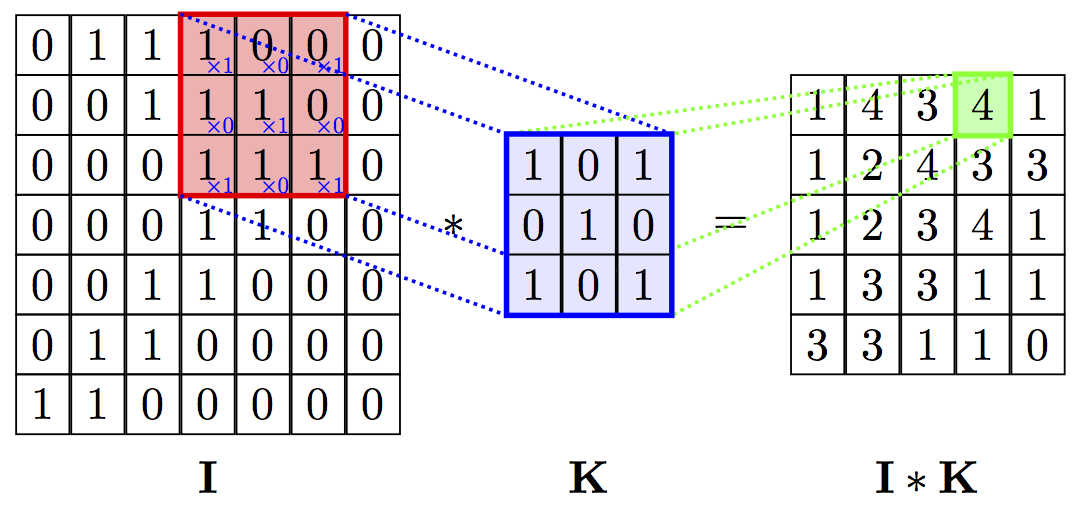
\includegraphics[width=0.9\textwidth]{convolution_example.png}
    \caption{Example of a convolution operation. Source: \url{https://github.com/PetarV-/TikZ}}
    \label{fig:conv_example}
\end{figure}

\subsection{Pooling}

When using CNNs, a pooling layer is also usually added after each convolutional layer. This pooling layer summarizes adjacent pixels, and it is used because it helps to achieve invariance and reduce the image of the output so that there are fewer parameters in the next layers \cite{bengio2015deep}. A very commonly used pooling function is \textbf{max pooling}, which returns the maximum value of a neighborhood of pixels. An example of max pooling is shown in figure \ref{fig:max_pool_example} for a $4 \times 4$ matrix, resulting in a $2 \times 2$ matrix after the function is applied.

\begin{figure}[H]
    \centering
    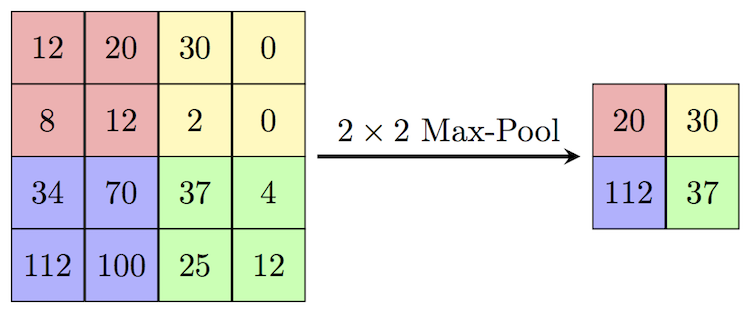
\includegraphics[width=0.6\textwidth]{max_pool_example.png}
    \caption{Example of max pooling function. Source: \url{https://computersciencewiki.org/index.php/File:MaxpoolSample2.png}}
    \label{fig:max_pool_example}
\end{figure}


\subsection{Architecture example}

To illustrate how all these concepts are put together, we will show an example of an architecture that is very commonly used in image classification problems, called \textbf{LeNet architecture}, introduced by \citeauthor{lecun1998gradient} in \citeyear{lecun1998gradient} for a digit classification problem \cite{lecun1998gradient}. The architecture assumes a grayscale input image of $32 \times 32$ pixels, which is then fed to 6 convolutional filters of size $5 \times 5$, each followed by an activation function and a $2 \times 2$ max pooling layer, then 16 convolutional filters of size $5 \times 5$, each with their corresponding activation functions and then the $2 \times 2$ max pooling layer, followed by two fully connected layers of sizes 120 and 84, and finally a softmax transformation to map to the 10 digit classification problem probabilities.

\begin{figure}[H]
    \centering
    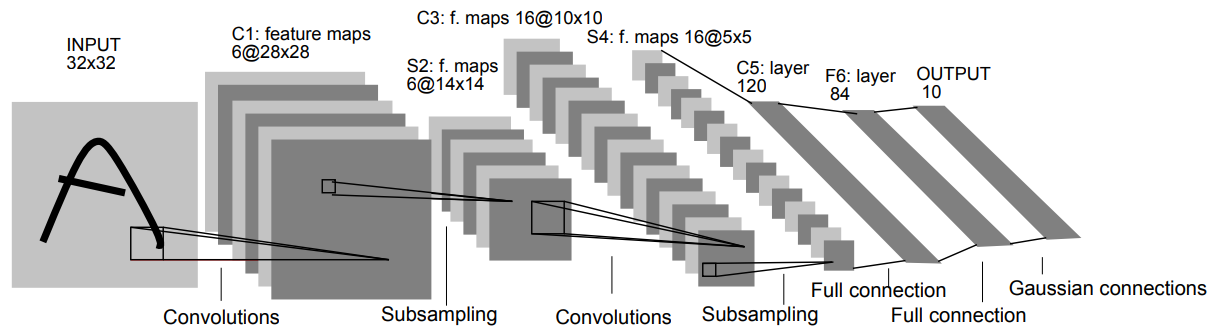
\includegraphics[width=\textwidth]{lenet.png}
    \caption{LeNet architecture (picture taken from \cite{lecun1998gradient}). The feature maps correspond to the convolutional filters and the subsampling refers to max pooling.}
    \label{fig:lenet_architecture}
\end{figure}
